\chapter{\label{ch:ml}Machine Learning Applications}
This chapter will discuss the machine learning approach taken in this project. First, a review of the data collected will be completed, this will outline the next steps taken. Next, the machine learning approach taken will be discussed, this will include an introduction to the adapted machine learning goal, identifying injury risks. This will be executed by replicating an approach developed for runners used by \textcite{Lovdal2021}, using the data provided by the literature.

\section{Rowing Data and training Review}
As discussed in \autoref{ch:data-collect-mng}, the data collected was limited to a small number of participants. This section will review the data collected, including the data sources used, the data collected, and the limitations of the data collected.
\subsection{Review of Data Available}
When the goals for the project were outlined, it was not clear what data was available, what data would be needed to produce a useful model, or how much data. In an attempt to have a larger set of data, the data collection system was built to require as little additional input from athletes as possible. As a result, the degree of context available for the data collected was limited. For example, session goals were not outlined, making it difficult to determine if a session was a hard session or an easy session. Additionally, gaps in training data could be present as a result of injury, illness, or athlete vacations. There was no way of collecting this information to discard these portions of data or account for gaps. Finally, most data was collected throughout the winter season. This part of a rower's yearly cycle is notorious for long periods of low-intensity training, with very few options to test performance. No clear performance "criterion" were recorded, making it difficult to even determine if a model was successful in predicting performance.

\subsection{Initial Machine Learning Plan}
Based on existing performance prediction literature, and before it became clear building a performance model with the data available was not feasible, an initial plan was formed to develop a model to predict performance. First, existing models would be adapted to rowing and implemented using the data collected. This would begin with implementing the more basic Banister fitness-fatigue model using the process outlined in \textcite{Morton1990}. Then a more complex model, such as PerPot \cite{perl2001}, would be implemented and evaluated. These two implementations of performance models would then be used to evaluate the effectiveness of any machine-learning-based models developed.

\subsection{Limitations of the Data and the Plan}
When this plan was devised, despite the lack of data available, there was a tentative strategy to combat the relative lack of data. As noted by \textcite{Churchill2014}, who only had three participants, the use of a hybrid ensemble of neural networks was effective in managing the relative lack of data. \textcite{Edelmannnusser2002} was also able to predict with strong accuracy a swimming performance using data from a single athlete. This optimistic approach to managing a small dataset further proved to be too ambitious. The "relative lack of data" experienced by Churchill still contained 250, 870, and 1107 days of training data for each of the three participants. Meanwhile, \textcite{Edelmannnusser2002} had 95 weeks of data for a single athlete, including 19 competitive performances. The data collected for this project was significantly less than these examples, with only 8 participants actively providing data throughout the data analysis stage, which only lasted about 3 months. While there were some erg tests completed during this period, some athletes were unable to complete these tests due to injury or illness, while other athletes did not log these efforts in detail, a limitation of the data collection system developed. Even if the data collection pipeline had been running for the full course of this project with the adjustments necessary to have a full set of features, not enough data would have been collected to develop a model to predict performance to any degree of accuracy.

\section{Developing an Injury Classification Model}
The limitations of the initial goal and plan described in the previous section resulted in a pivot to a new goal. Given the limitations of the data collected for training a machine-learning model, it became necessary to look for a dataset that could be used to develop a modeling approach that could be applied to rowing data. Fortunately, \textcite{Lovdal2021} explored the use of machine learning to predict injuries using binary classification, with the full dataset published alongside the paper. 

This section will outline the steps taken to replicate the model, including the data used, the model iteration and development, the evaluation of the model, and a reflection on its potential applicability to rowing data.

\subsection{Predicting Injury in Runners}
\subsubsection{Data review}
The data provided by \textcite{Lovdal2021} the training log of a high-performance Dutch running squad over the course of 7 years (2012-2019) containing 77 middle- and long-distance athletes. These athletes compete at distances between 800m and full marathon distances, the training for both disciplines is largely endurance-focused so training programs are relatively the same. Furthermore, the training program remained the same as the team's head coach remained consistent throughout the 7-year period. The dataset has also been pre-cleaned. Injuries were flagged in the dataset by athletes being either unable to start or complete a session. These flags were then considered an injury event if an athlete had been training injury-free for the previous 3 weeks. Healthy events were those where an athlete was fully fit 3 weeks before and 3 weeks after the event day. Events that contained missing or anomalous data were removed from the dataset. Recurring injury events, those occurring within 3 weeks of a previous injury event, were also removed from the dataset.

This cleaning process resulted in a dataset containing 74 athletes, 42,183 healthy and 583 injury events for the day-to-day model, and 42,223 healthy and 575 injury events for the week-to-week model. The number of injuries per athlete ranges from 0 to 35.

It is evident this data set is quite comprehensive, with detailed information about training behaviours, and a clear definition of injury; this data set is ideal for developing a model to predict injury risk. Furthermore, with many of the same potential features as a complete rowing dataset would contain, the approaches used to predict injury risk in this dataset could be applied to rowing data.

\subsubsection{Model Development}
There are a number of approaches which can be taken when developing a classification model. First, an understanding of the problem is crucial. Different classification models and algorithms are better suited to different kinds of problems or expected outcomes. For example, a decision tree model is better suited to problems where the relationships between features are non-linear, while a logistic regression model is better suited to problems where the relationships between features are linear. Given the non-linear relationships between training features and injury risk, and the importance of understanding feature ranking (ie. what behaviours lead to higher injury risk), a decision tree model approach is best suited for this problem. When using a decision tree approach, using ensemble learning (ie. an approach that combines multiple models to produce the most accurate result), is also recommended. This is because decision trees are prone to overfitting, and ensemble learning can help to reduce this risk and illicit more general results.

Based on the considerations above, the Extreme Gradient Boosting, or XGBoost, algorithm was used. This decision tree boosting system has performed well in a number of classification problems \cite{Lovdal2021}, and is well suited to the problem of predicting injury risk. 

The next step in developing the model was to select training and validation data. Given the unbalanced nature of injury data in training, two steps were taken to ensure the model was trained on balanced data. First, a balanced subset of the data was selected at random, with replacement, from the training set. Next, a bagging approach was used to train the model on the balanced subsets of the data. This approach was used to ensure the model was not biased towards predicting healthy events and was able to predict injury events with a high degree of accuracy. 

When implementing the XGBoost algorithm, a number of parameters are passed to the classifier. The only parameters explicitly passed to the classifier are the learning rate, the maximum depth of the tree, and the number of trees, with the remaining parameters being left at default values. A low learning rate of $0.01$ was passed, a choice of ${2, 3}$ was selected for the maximum depth of the tree, and the number of trees ${256, 512}$ was selected. \textcite{Lovdal2021} did not fine-tune any of the participating models, only adjusting the values described.

The final step of making a usable model was to perform some calibration. This step transforms the output of the model so that a risk score can be generated for each athlete event. This risk score can then be used to determine the likelihood of an injury event occurring. This was done by fitting a logistic regression model -- using \texttt{CalibratedClassifierCV} from the \texttt{scikitlearn} package -- to the output of the XGBoost model. This model was then used to generate a risk score for each athlete event. Finally, a threshold needed to be selected to classify a predicted event as an injury event or not. When selecting the threshold value, it is important to consider the cost of false positives and false negatives. In this case, a threshold value that results in more false negatives (ie. predicting an injury event when there is none) is preferred, as the cost of a false positive (ie. not predicting an injury event when there is one) is higher. Practically, taking a day off training to mitigate a potential injury is less costly than training resulting in an injury. An injury will result in more days taken off, likely a longer recovery period, and as a result a loss of performance. 

\subsubsection{Model Evaluation}
Evaluating the accuracy and effectiveness of a classification model is arguably the most important step in developing the model. When evaluating this model it is important to understand what the model is predicting, and how well it is predicting it. To evaluate this model, the area under the receiver operating characteristic curve (AUC-ROC) was used. This metric is a measure of how well the model can distinguish between injury and healthy events. The AUC-ROC ranges from 0 to 1, with a value of 0.5 indicating the model is no better than random, and a value of 1 indicating the model is perfect. In sports science, an AUC of 0.7 is considered strong evidence of a model's predictive ability \cite{Lovdal2021}. 

\begin{figure}[ht]
  \centering
  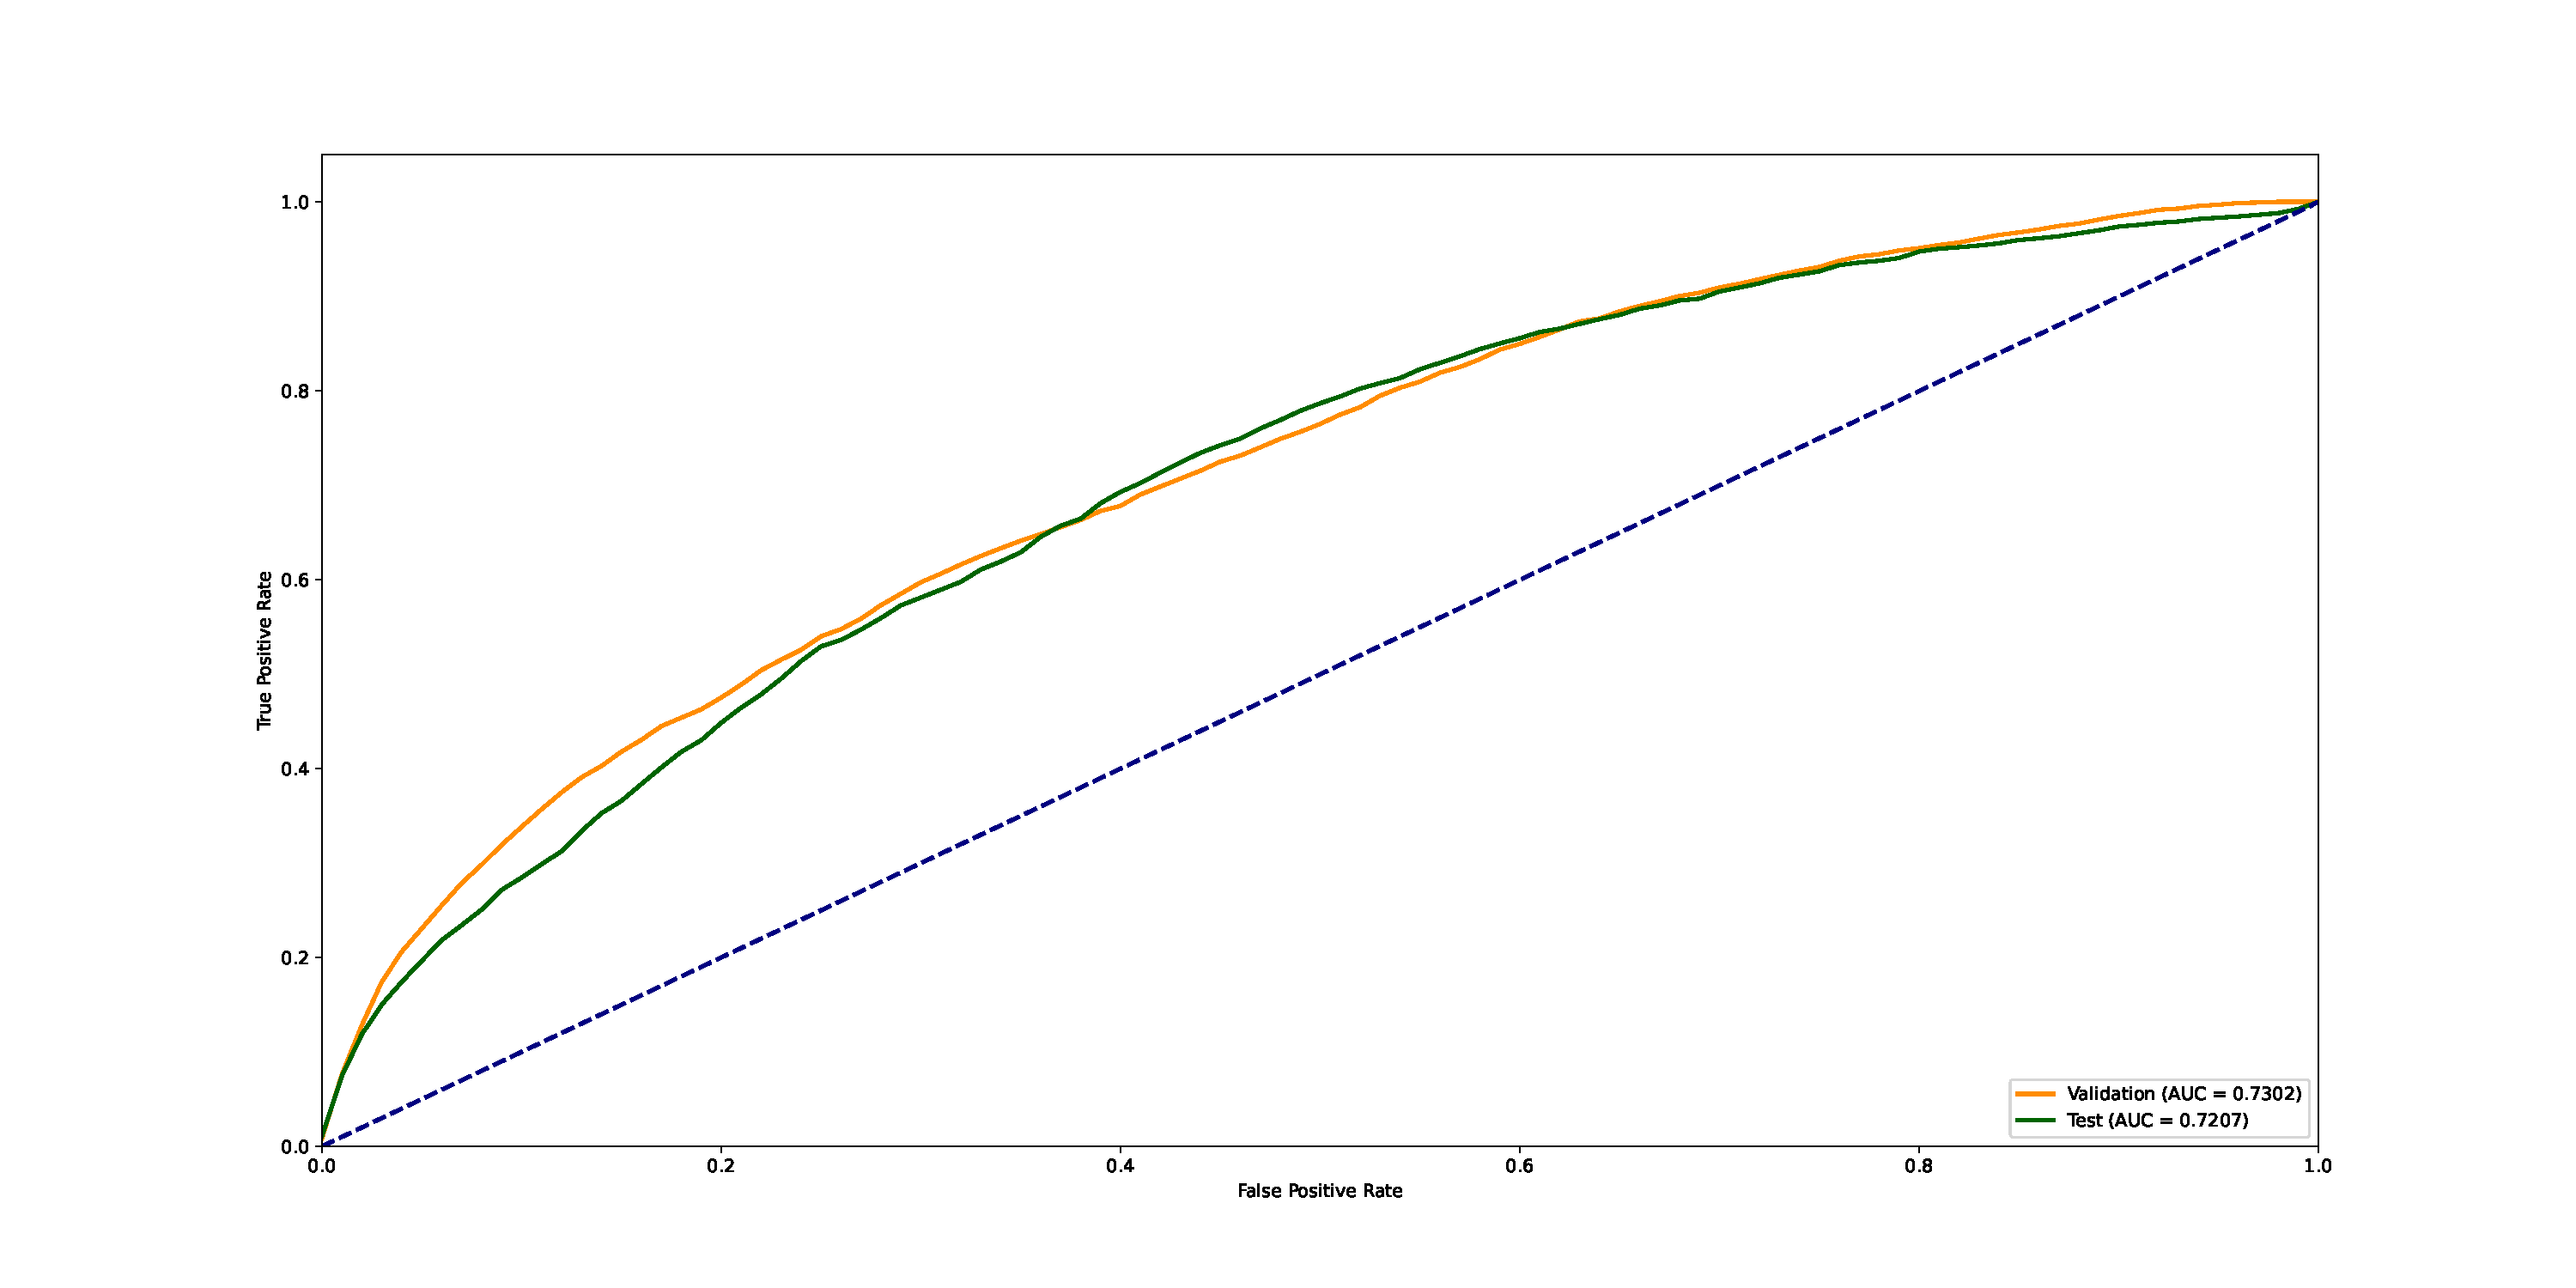
\includegraphics[width=\textwidth]{figures/day_ROC.pdf}
  \captionsetup{justification=centering,width=0.8\textwidth}
  \caption[Runner Injury Day Model ROC Curve]{\label{fig:day_roc}The receiver operating characteristic curve for the runner injury classifier trained on daily data leading into the injury event.}
\end{figure}
\begin{figure}[ht]
  \centering
  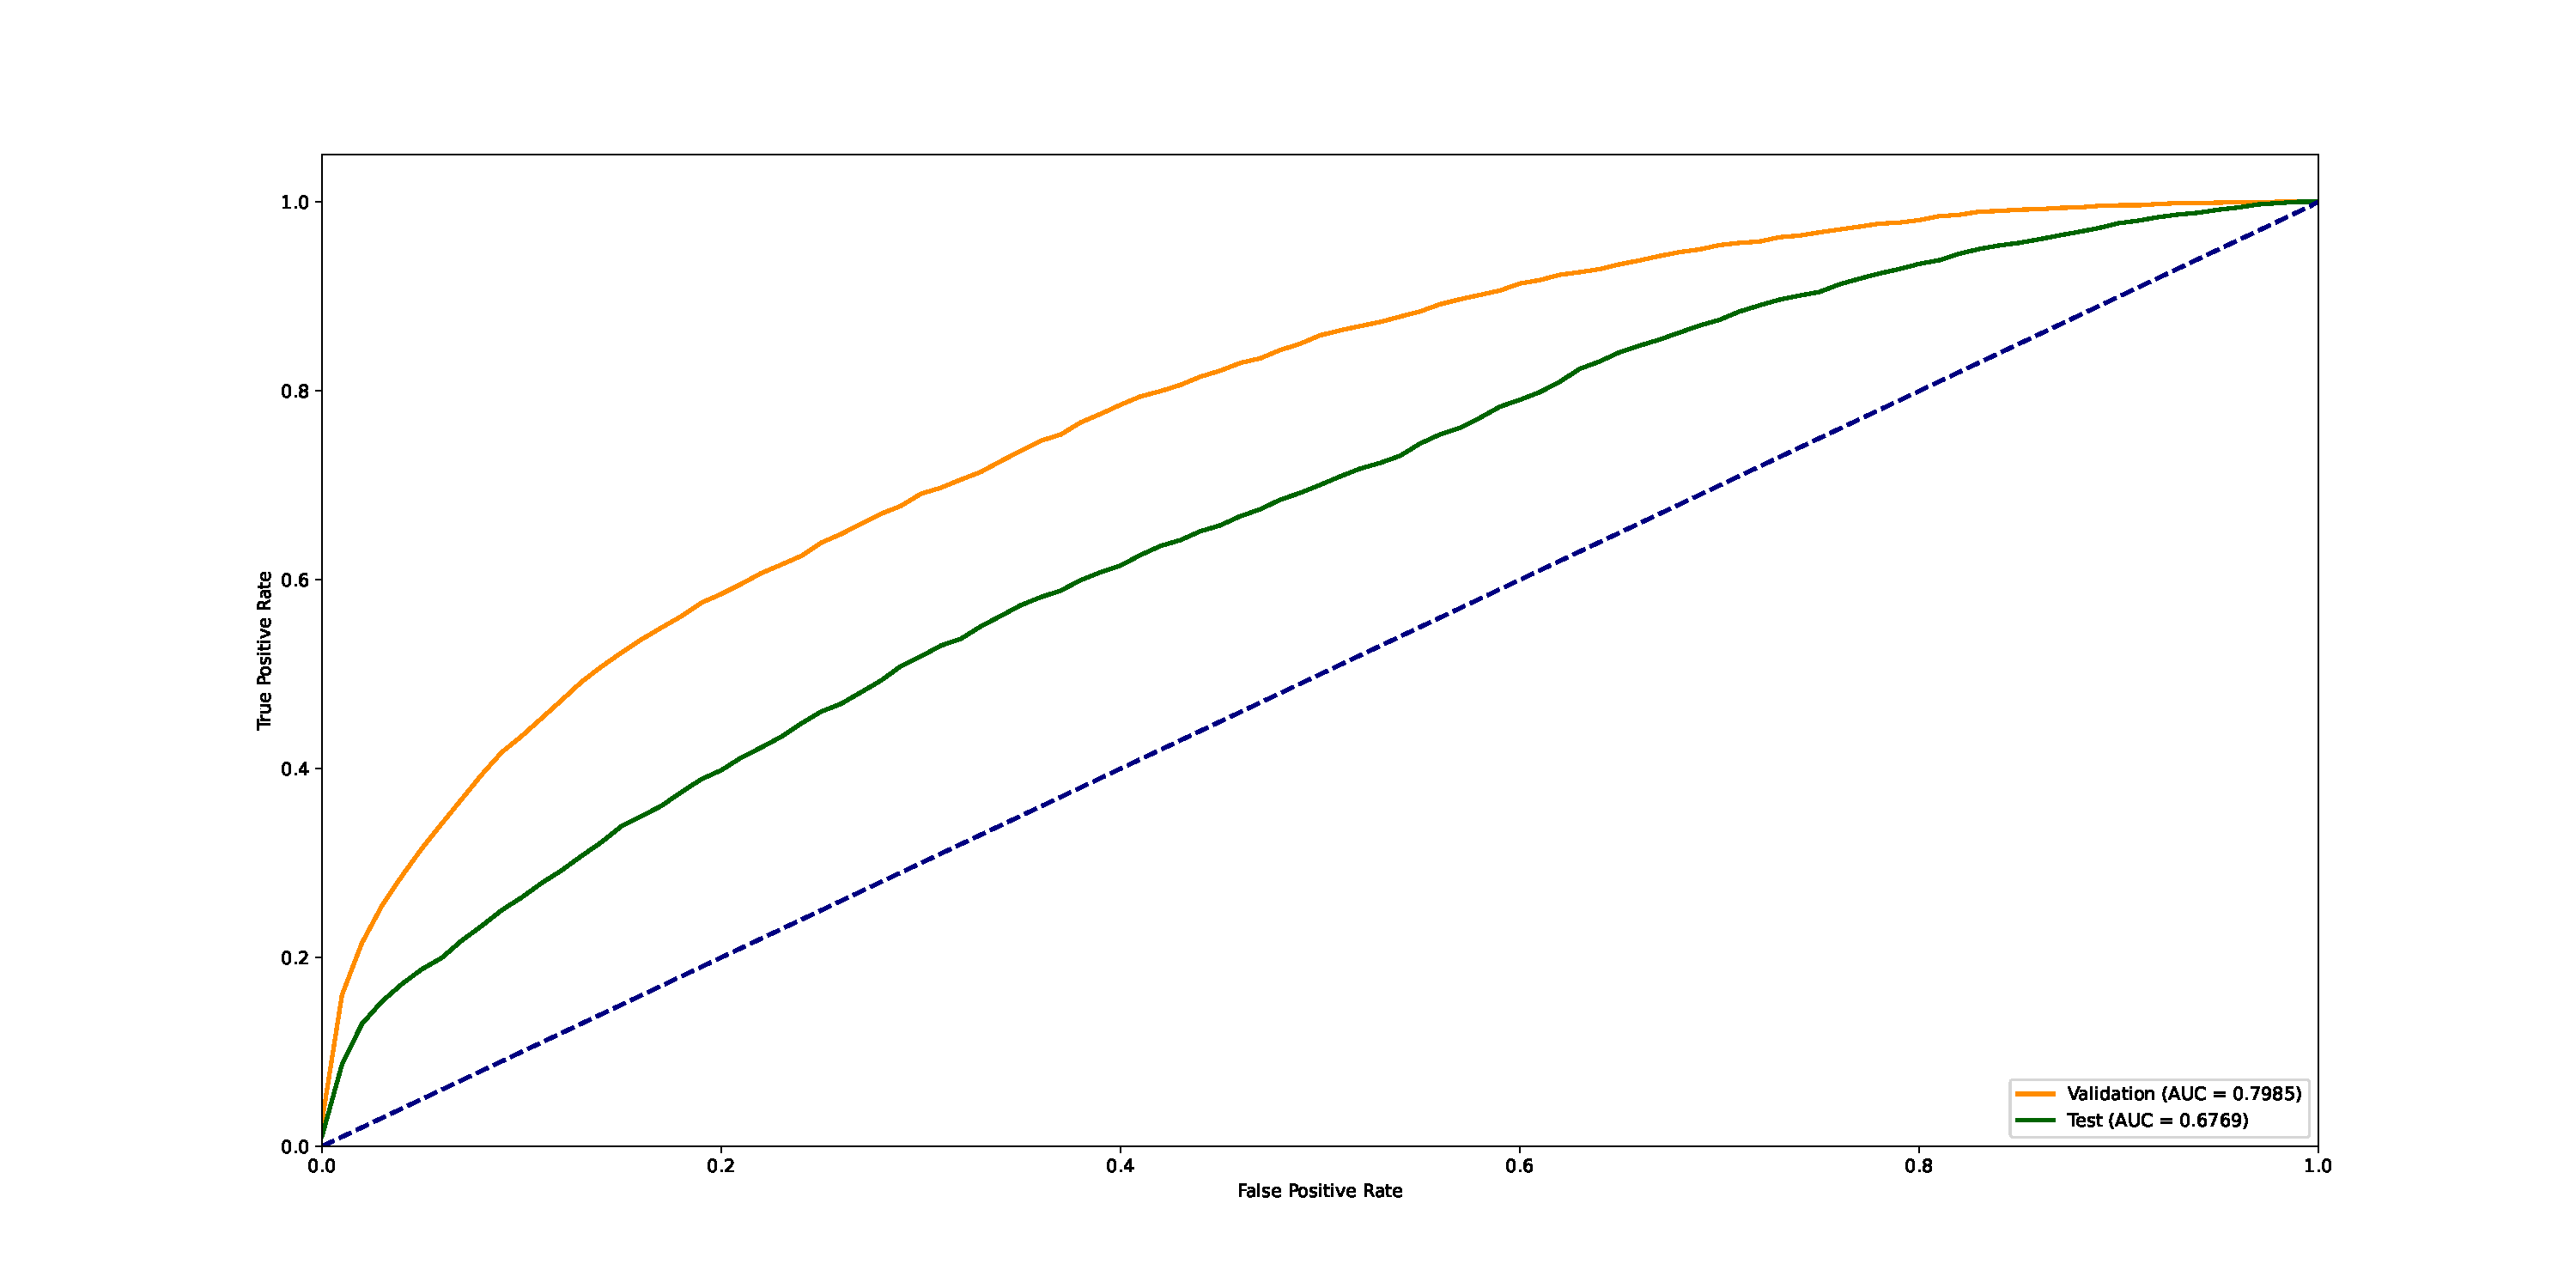
\includegraphics[width=\textwidth]{figures/week_ROC.pdf}
  \captionsetup{justification=centering,width=0.8\textwidth}
  \caption[Runner Injury Day Model ROC Curve]{\label{fig:week_roc}The receiver operating characteristic curve for the runner injury classifier trained on weekly data leading into the injury event.}
\end{figure}

For this implementation of the XGBoost Classifier, both approaches taken by \textcite{Lovdal2021} were implemented, the day-to-day model and the week-to-week model. The day-to-day model was trained on data considering the 7-day period leading up to an injury event, while the week-to-week model was trained on data considering the 4-week period leading up to an injury event. The ROC curves for the day model and week model can be seen in \ref{fig:day_roc} and \ref{fig:week_roc} respectively. The average AUC values for the day model were 0.73 and 0.72 for the validation and test data, while the average AUC values for the week model were 0.79 and 0.71 for the validation and test data, respectively. The consistency between the observed AUC for both models demonstrates the ability of each model to generalise, and new (unseen) data is correctly classified.

\begin{table}[hb]
  \centering
  \captionsetup{labelfont=bf,textfont=bf}
  \caption[Runner Injury Prevention Approach Comparison]{Mean (SD) Test Scores Obtained by 5 Experiments, With a Threshold of 0.445 for the Day Approach and 0.462 for the Week Approach}
  \label{tab:ml_results}
  \begin{tabularx}{\textwidth}{@{}l *{3}{Y}@{}}
    \toprule
    \textbf{Approach} & \textbf{Specificity} & \textbf{Sensitivity} & \textbf{AUC} \\ \midrule
    Day & 0.746 (0.02) & 0.564 (0.07) & 0.73 (0.002) \\
    Week & 0.723 (0.01) & 0.545 (0.04) & 0.68 (0.006) \\ \bottomrule
  \end{tabularx}%
\end{table}

To further evaluate the models, reviewing the specificity and sensitivity of the model is important. The specificity of a model is the proportion of true negatives that are correctly identified, while the sensitivity of a model is the proportion of true positives that are correctly identified. Simply put, the specificity ratio shows: of all healthy events predicted, how many were correct, while the sensitivity ratio shows: of all injury events, how many were identified. A breakdown of the results can be seen in \autoref{tab:ml_results}. Based on these results, the day model performs better. This is likely due to the accumulated impact of acute training load on injury risk, which is more accurately captured by the day model. The week model, on the other hand, may not capture the acute training load as well, leading to a lower sensitivity and specificity. The day model has a noticeably higher AUC, indicating better potential performance on new data.

Finally, as a result of using a decision tree-based approach for classification, a feature ranking for each model was generated. This feature ranking can be used to identify which features are most important in predicting injury events, and can be used to inform future training programs, this is available in the appendix (\autoref{fig:app_day_features}, \autoref{fig:app_week_features}).


\subsection{Applying the Model to Rowing Data}
Based on the evaluated effectiveness of the above model on running training data, the potential application for rowing data is promising. Furthermore, a brief anecdotal analysis of the feature ranking for the more effective day model shows that the most important features are related to the acute training load. The ability for this model to uncover complex relationships between training features and injury risk is promising for the application of this model to rowing data. Finally, the training data available to be collected from rowing training is quite similar to the training data collected from running training, with the same potential features available. This model could be applied to rowing data with minimal changes, and could be used to predict injury risk in rowers.